% !TeX program = xelatex
%-------------------------------------------------------------------------------------------------
% گزارش پیشرفت پروژه: توسعه‌ی الگوریتم SCL-Star به ESCL-Star
% این فایل مستقل است و با ساختار و قواعد نگارشی رساله‌ی tehran-thesis (فصل روش تحقیق و فصل نتایج)
% نوشته شده است: عنوان‌بندی فارسی، قاعده‌ی «ارجاع به جلو» برای اشکال/جداول/الگوریتم‌ها، استفاده از
% \lr برای اصطلاحات لاتین، و کدگذاری الگوریتم‌ها با محیط algorithmic.
% کامپایل: xelatex نیازمند فونت فارسی (مطابق پیکربندی tehran-thesis/tex/commands.tex) است.
%-------------------------------------------------------------------------------------------------
\documentclass[a4paper,12pt]{article}

\usepackage{amsthm,amssymb,amsmath}
\usepackage[a4paper, top=30mm, bottom=30mm, outer=20mm, inner=25mm]{geometry}
\usepackage[final]{graphicx}
\graphicspath{{../}}
\usepackage{tabularx}
\usepackage{booktabs}
\usepackage{float}
\usepackage[usenames,dvipsnames,svgnames,table]{xcolor}
\usepackage{algorithm}
\usepackage{algorithmic}
\numberwithin{algorithm}{section}

% فراخوانی زی‌پرشین (باید آخرین بسته باشد، مطابق قاعده‌ی tehran-thesis)
\usepackage[extrafootnotefeatures, localize=on, displaymathdigits=persian]{xepersian}
% قلم‌های فارسی/لاتین tehran-thesis (پوشه‌ی font/ کنار این گزارش)، زیرا Noto Naskh Arabic
% فاقد گلیف‌های نویسه‌های لاتینِ رایج (پرانتز، بولت، خط‌فاصله‌ی طولانی و...) است و باعث
% خطای «Missing character» در سراسر سند می‌شد.
\settextfont[Path={./font/}, BoldFont={XB NiloofarBd.ttf}, ItalicFont={XB NiloofarIt.ttf}, BoldItalicFont={XB NiloofarBdIt.ttf}]{XB Niloofar.ttf}
\setlatintextfont[Path={./font/}, BoldFont={Junicode-Bold.ttf}, ItalicFont={Junicode-Italic.ttf}, BoldItalicFont={Junicode-BoldItalic.ttf}]{Junicode.ttf}
\setdigitfont[Path={./font/}]{XB Niloofar.ttf}

\usepackage[unicode=true,colorlinks,linkcolor=blue,citecolor=blue,urlcolor=blue,final]{hyperref}

% رفعِ ناسازگاریِ tabularx با xepersian (بدون این خط، \end{tabularx} در سند
% فارسی به خطای «Undefined control sequence» برای \UseMathForPositioningText می‌انجامد)
\makeatletter
\providecommand\UseMathForPositioningText{}
\makeatother

% ترجمه‌ی کامل کلیدواژه‌های محیط algorithmic به فارسی (مطابق tehran-thesis/tex/commands.tex)
\renewcommand{\algorithmicrequire}{\textbf{ورودی:}}
\renewcommand{\algorithmicensure}{\textbf{خروجی:}}
\renewcommand{\algorithmicend}{\textbf{پایان}}
\renewcommand{\algorithmicif}{\textbf{اگر}}
\renewcommand{\algorithmicthen}{\textbf{آنگاه}}
\renewcommand{\algorithmicelse}{\textbf{وگرنه}}
\renewcommand{\algorithmicfor}{\textbf{برای}}
\renewcommand{\algorithmicforall}{\textbf{برای هر}}
\renewcommand{\algorithmicdo}{\textbf{انجام بده}}
\renewcommand{\algorithmicwhile}{\textbf{تا زمانی که}}
\renewcommand{\algorithmicloop}{\textbf{تکرار کن}}
\renewcommand{\algorithmicrepeat}{\textbf{تکرار کن}}
\renewcommand{\algorithmicuntil}{\textbf{تا زمانی که}}
\renewcommand{\algorithmicprint}{\textbf{چاپ کن}}
\renewcommand{\algorithmicreturn}{\textbf{بازگردان}}
\renewcommand{\algorithmicand}{\textbf{و}}
\renewcommand{\algorithmicor}{\textbf{یا}}
\renewcommand{\algorithmicnot}{\textbf{نقیض}}
\renewcommand{\algorithmicto}{\textbf{تا}}
\renewcommand{\algorithmictrue}{\textbf{درست}}
\renewcommand{\algorithmicfalse}{\textbf{نادرست}}
\renewcommand{\algorithmicendif}{\algorithmicend\textbf{ شرط }\algorithmicif}
\renewcommand{\algorithmicendfor}{\algorithmicend\textbf{ حلقه‌ی }\algorithmicfor}
\renewcommand{\algorithmicendwhile}{\algorithmicend\textbf{ حلقه‌ی }\algorithmicwhile}
\renewcommand{\algorithmicendloop}{\algorithmicend\textbf{ حلقه‌ی }\algorithmicloop}
\renewcommand{\algorithmiccomment}[1]{\{{\itshape #1}\}}
\def\listalgorithmname{فهرست الگوریتم‌ها}

\title{گزارش پیشرفت پروژه:\\ توسعه‌ی الگوریتم \lr{SCL-Star} به \lr{ESCL-Star} و تعمیم تولیدکننده‌ی آزمون‌های خودکار}
\author{آرین باستانی}
\date{}

\begin{document}
\pagenumbering{arabic}
\maketitle

\begin{abstract}
این گزارش، توسعه‌ی الگوریتم یادگیریِ ترکیبیِ \lr{SCL-Star} به \lr{ESCL-Star} را مستند می‌کند: تعمیمی که به کنش‌های هم‌گام‌ساز اجازه می‌دهد به‌جای یک خروجیِ ایستایِ ثابت، خروجی‌های متفاوت اما سازگار در نقاط هم‌گامی تولید کنند. علاوه بر شرح صوری و پیاده‌سازیِ الگوریتم، تعمیمِ متناظرِ تولیدکننده‌ی آزمون‌های خودکار نیز با جزئیات کامل ارائه می‌شود. در پایان، نتایج آزمایش‌ها روی آزمون‌های تولیدی برای چهار توپولوژی و نیز یک بنچمارک واقعیِ تازه (\lr{bankCard}) گزارش می‌شود که نشان می‌دهد مزیتِ یادگیریِ ترکیبی نسبت به یادگیریِ یکپارچه، پس از این تعمیم همچنان حفظ می‌شود.
\end{abstract}

\tableofcontents
\listoffigures
\listoftables
\listofalgorithms
\clearpage

\section{مقدمه}
این گزارش، توسعه‌هایی را مستند می‌کند که از تعهد \lr{4844f2f}\LTRfootnote{4844f2f754af13a63b5aacaad668fd637572c339} تا انتهای تاریخچه‌ی فعلی مخزن \lr{ESCL-Star} پیاده‌سازی شده‌اند. محور اصلی کار، رفع یک محدودیت بنیادین در الگوریتم یادگیری ترکیبی \lr{SCL-Star}\LTRfootnote{Synchronous Compositional Learning} است: در نگارش پیشین، هر کنش هم‌گام‌ساز\LTRfootnote{synchronizing action} می‌بایست در تمام مؤلفه‌ها و در تمام حالت‌هایی که رخ می‌دهد، دقیقاً یک خروجی ایستا و یکسان تولید کند. الگوریتم توسعه‌یافته که در این گزارش \lr{ESCL-Star}\LTRfootnote{Extended SCL-Star} نامیده می‌شود، این محدودیت را برمی‌دارد و اجازه می‌دهد یک کنش هم‌گام‌ساز، در نقاط مختلف اجرای سامانه، خروجی‌های متفاوتی داشته باشد؛ به شرط آنکه در هر لحظه‌ی هم‌گامی، تمام مؤلفه‌های شرکت‌کننده در آن هم‌گامی، خروجی یکسانی برای آن کنش تولید کنند. این شرط، برای حفظ قطعیت\LTRfootnote{determinism} ترکیب موازی سامانه‌ی هدف ضروری است.

پس از تشریح الگوریتم \lr{ESCL-Star}، گزارش به بخش دوم و پراهمیت‌تر کار می‌پردازد: تعمیم تولیدکننده‌ی آزمون‌های خودکار\LTRfootnote{Generated Tests} به‌گونه‌ای که بتواند مؤلفه‌های تصادفی‌ای تولید کند که کنش‌های هم‌گام‌ساز آن‌ها می‌توانند خروجی‌های متفاوت داشته باشند، اما همواره در نقاط هم‌گامی با یکدیگر سازگارند. طراحی این تولیدکننده از دشوارترین بخش‌های این کار بوده و در بخش \ref{sec:generator} با جزئیات کامل تشریح می‌شود. در پایان، نتایج آزمایش‌های اجراشده روی آزمون‌های تولیدی و همچنین یک بنچمارک واقعی جدید (\lr{bankCard}) گزارش می‌شود.

\section{مروری بر محدودیت الگوریتم پیشین}
در \lr{SCL-Star}، سامانه‌ی هدف $M=\parallel_{i=1}^{n}M_i$ متشکل از $n$ مؤلفه‌ی موازیِ هم‌گام است. الگوریتم به‌صورت برخط\LTRfootnote{on-the-fly} یک پوشش $I^F=\{I_1,\dots,I_n\}$ از الفبای کل سامانه را می‌سازد؛ اگر دو مجموعه‌ی $I_i$ و $I_j$ اشتراک غیرتهی داشته باشند، مؤلفه‌های متناظر روی کنش‌های مشترک هم‌گام می‌شوند. فرض بنیادین نگارش پیشین آن بود که هر کنش هم‌گام‌ساز، خروجی واحدی دارد که در تمام مؤلفه‌ها و تمام حالت‌ها ثابت است (مثلاً کنش «\lr{a}» همیشه خروجی «\lr{1}» تولید می‌کند). این فرض، تشخیصِ نادرستی کنش‌های هم‌گام‌ساز را ساده می‌کرد: کافی بود در طول یادگیری، خروجی هر کنش هم‌گام‌ساز رصد و در صورت مشاهده‌ی هر مقدار متفاوت، فوراً آن کنش از مجموعه‌ی \lr{sync} حذف شود.

این فرض در عمل بسیاری از سامانه‌های واقعی را پوشش نمی‌دهد؛ برای نمونه، در پروتکل‌های کارت بانکی (بخش \ref{sec:bankcard})، یک کنش می‌تواند بسته به وضعیت داخلی مؤلفه (مثلاً وضعیت احراز هویت) پاسخ‌های متفاوتی صادر کند، در حالی که همچنان کنشی هم‌گام‌ساز میان چند مؤلفه محسوب می‌شود. هدف این پروژه، تعمیم الگوریتم برای پوشش چنین رفتاری بدون از دست دادن قطعیت مدل ترکیبی بود.

\section{الگوریتم \lr{ESCL-Star}}\label{sec:escl}

\subsection{ایده‌ی اصلی}
در \lr{ESCL-Star} کنش هم‌گام‌ساز $u$ مجاز است در نقاط مختلف اجرا، خروجی‌های متفاوتی تولید کند؛ تنها الزام آن است که هرگاه دو یا چند مؤلفه هم‌زمان روی $u$ هم‌گام می‌شوند، خروجیِ تولیدی هر یک از آن‌ها برای $u$ در آن نقطه‌ی هم‌گامی، دقیقاً برابر باشد. این شرط، عدم‌قطعیتِ خروجی در ترکیب موازی دو ماشین \lr{Mealy} قطعی را از بین می‌برد و ضامن صحت ترکیب است.

از منظر پیاده‌سازی، تفاوت اصلی با نگارش پیشین در نحوه‌ی پردازش ضدمثال\LTRfootnote{counter-example} است. در نگارش پیشین، به محض مشاهده‌ی دو خروجی متفاوت برای یک کنش هم‌گام‌ساز، آن کنش به‌سادگی از \lr{sync} حذف می‌شد (شکل \ref{fig:old-alg}). این کار در حالتی که کنش واقعاً هم‌گام‌ساز است اما خروجی پویا دارد، اشتباه است؛ زیرا کنش را به غلط ناهم‌گام تشخیص می‌دهد. در \lr{ESCL-Star} (شکل \ref{fig:new-alg} برای پیش‌نویس اولیه، و پیاده‌سازی نهایی در بخش \ref{sec:impl})، به‌جای حذف کنش از \lr{sync}، مجموعه‌های الفبایی\LTRfootnote{input sets} حاوی آن کنش را می‌یابیم و آن‌ها را \emph{با هم} یاد می‌گیریم؛ در صورتی که خروجیِ کنش هنگام هم‌گامی در مدل یادگرفته‌شده‌ی ترکیبی هم‌چنان ناسازگار باشد، آنگاه واقعاً کنش هم‌گام‌ساز نیست و مجموعه‌های الفبایی متناظر با آن باید ادغام شوند تا در یک مؤلفه‌ی واحد یاد گرفته شوند.

\begin{figure}[H]
\centering
\includegraphics[width=0.85\textwidth]{Algs/Old.jpg}
\caption{الگوریتم پردازش ضدمثال در \lr{SCL-Star}: به‌محض مشاهده‌ی یک خروجی متفاوت برای کنش هم‌گام‌ساز $u$، کنش بدون بررسی بیشتر از \lr{sync} حذف می‌شود.}
\label{fig:old-alg}
\end{figure}

\begin{figure}[H]
\centering
\includegraphics[width=0.85\textwidth]{Algs/New.jpg}
\caption{پیش‌نویس اولیه‌ی الگوریتم پردازش ضدمثال در \lr{ESCL-Star}: به‌جای حذف کنش، مجموعه‌های الفبایی مرتبط با آن یاد گرفته و صحت هم‌گامی آن‌ها با \lr{LearnSyncSets} بررسی می‌شود.}
\label{fig:new-alg}
\end{figure}

\subsection{تعاریف پایه}
\begin{itemize}
	\item \textbf{\lr{SymbolsSet}}: مجموعه‌ی تمام کنش‌های متمایز حاضر در یک ضدمثال \lr{CE} را برمی‌گرداند.
	\item \textbf{\lr{DependentSets}}: از میان پوشش $I^F$، مجموعه‌هایی را برمی‌گرداند که حداقل یک کنش مشترک با یک مجموعه‌ی داده‌شده دارند.
	\item \textbf{\lr{Merge}}: دو پوشش را می‌گیرد و مجموعه‌های مشترکشان را با اجتماع آن‌ها جایگزین می‌کند.
	\item \textbf{\lr{LearnSyncInParts}}: هر مجموعه‌ی الفبایی $I_i\in I^F$ را با \lr{L*} به‌طور مستقل یاد می‌گیرد و ترکیب موازی هم‌گام آن‌ها را برمی‌گرداند.
\end{itemize}

\subsection{پیاده‌سازی نهایی: \lr{makeSet}، \lr{merge} و \lr{ProductMealy}}\label{sec:impl}
پیاده‌سازی نهایی در فایل \lr{src/main/SclStar.java} این ایده را در سه گام به‌کار می‌بندد که در الگوریتم \ref{alg:processce} خلاصه شده است:

\begin{enumerate}
	\item تابع \lr{makeSet} مجموعه‌ی $I_{CE}$ را از تمام کنش‌های متمایز حاضر در ضدمثال کمینه\LTRfootnote{minimal counter-example} می‌سازد و آن را جایگزین هر مجموعه‌ی موجود در $I^F$ می‌کند که زیرمجموعه‌ی آن است.
	\item مجموعه‌های $I^F$ که با $I_{CE}$ اشتراک دارند اما با آن برابر نیستند، به‌عنوان $I^D$ (مجموعه‌های وابسته‌ی مشکوک) جدا می‌شوند.
	\item اگر $I^D$ ناتهی باشد، \lr{learnSynSets} فراخوانی می‌شود: هر مجموعه در $I^D\cup\{I_{CE}\}$ به‌طور مستقل با \lr{L*} یاد گرفته و توسط \lr{ProductMealy.mergeFSMs} در قالب یک ترکیب هم‌گام واحد ساخته می‌شود. در حین ساخت این ترکیب، هرگاه یک کنش مشترک $a$ در دو مدل جزئی، برای یک حالتِ مشترکِ ترکیب‌شده، دو خروجی متفاوت تولید کند، آن کنش به فهرست \lr{wrongSyncs} افزوده می‌شود (این بررسی دقیقاً معادل تابع \lr{CheckOutputs} در تعریف صوری الگوریتم است).
	\item برای هر کنش در \lr{wrongSyncs}، مجموعه‌های الفبایی حاوی آن (از طریق \lr{DependentSets}) گرد آورده و با \lr{merge} در $I^F$ ادغام می‌شوند تا از این پس با هم و در قالب یک مؤلفه‌ی یادگیری واحد آموخته شوند.
\end{enumerate}

\begin{algorithm}[H]
\caption{پردازش ضدمثال در \lr{ESCL-Star} (خلاصه‌ی پیاده‌سازی \lr{ProcessCE})}
\label{alg:processce}
\begin{algorithmic}[1]
\REQUIRE ضدمثال کمینه $CE$، پوشش فعلی $I^F$
\ENSURE پوشش به‌روزشده‌ی $I^F$
\STATE $I_{CE} \leftarrow \text{\lr{makeSet}}(CE)$
\IF{$\exists I_i \in I^F$ به‌طوری‌که $I_i \subseteq I_{CE}$}
    \STATE $I^F \leftarrow I^F \setminus \{I_i\}$
\ENDIF
\STATE $I^F \leftarrow I^F \cup \{I_{CE}\}$
\STATE $I^D \leftarrow \{I_j \in I^F \mid I_j \neq I_{CE} \wedge I_j \cap I_{CE} \neq \emptyset\}$
\IF{$I^D \neq \emptyset$}
    \STATE $\mathcal{H} \leftarrow \text{\lr{LearnSyncInParts}}(M,\, I^D \cup \{I_{CE}\})$ \COMMENT{یادگیری جزئی هر مجموعه با \lr{L*}}
    \STATE $\text{\lr{wrongSyncs}} \leftarrow$ کنش‌های هم‌گامی که در ساخت \lr{ProductMealy} خروجی ناسازگار داشته‌اند
    \STATE $I^{D'} \leftarrow \bigcup_{u \in \text{\lr{wrongSyncs}}} \text{\lr{DependentSets}}(I^D \cup \{I_{CE}\},\, u)$
    \FOR{هر $I_i \in I^{D'}$}
        \STATE $I^F \leftarrow \text{\lr{Merge}}(I^F,\, I_i)$
    \ENDFOR
\ENDIF
\RETURN $I^F$
\end{algorithmic}
\end{algorithm}

نکته‌ی کلیدی آن است که ادغام دیگر بر پایه‌ی «هر خروجی متفاوت برابر است با ناهم‌گام‌سازی» صورت نمی‌گیرد؛ بلکه فقط زمانی رخ می‌دهد که خروجیِ ناسازگار، در \emph{لحظه‌ی واقعیِ هم‌گامی دو مؤلفه‌ی مستقلاً یادگرفته‌شده} ظاهر شود. این تغییر، دقیقاً همان چیزی است که امکان یادگیری صحیح سامانه‌هایی با کنش‌های هم‌گام‌سازِ چندخروجی را فراهم می‌کند.

\section{تعمیم تولیدکننده‌ی آزمون‌های خودکار}\label{sec:generator}
پس از تعمیم الگوریتم یادگیری، لازم بود مجموعه‌ای از آزمون‌های خودکار ساخته شود که واقعاً رفتار موردنظر (کنش هم‌گام‌ساز با خروجی پویا اما سازگار در نقاط هم‌گامی) را در خود داشته باشند؛ در غیر این صورت امکان سنجش عملکرد \lr{ESCL-Star} در برابر این حالت جدید وجود نداشت. طراحی این تولیدکننده، به‌مراتب پیچیده‌تر از توسعه‌ی الگوریتم یادگیری بود و در این بخش با جزئیت کامل شرح داده می‌شود.

\subsection{صورت‌مسئله}
هر مؤلفه‌ی هم‌گام‌ساز باید به‌طور کاملاً مستقل و تصادفی تولید شود (توپولوژی، تعداد حالت‌ها، کنش‌های خصوصی\LTRfootnote{unsynch acts} دلخواه)، اما \emph{ردِ خروجی}\LTRfootnote{output trace} کنش هم‌گام‌ساز مشترک، از حالت آغازین به بعد، باید در همه‌ی مؤلفه‌های شرکت‌کننده در آن هم‌گامی، دقیقاً یکسان باشد. از آنجا که هر ماشین حالت متناهی قطعی، در نهایت به یک چرخه‌ی دوره‌ای می‌رسد، رَدِ خروجیِ یک کنش را می‌توان با یک الگو\LTRfootnote{pattern} به‌صورت زوج (پیشوند، دوره‌ی تناوب) نمایش داد:
\[
\text{\lr{pattern}} = (\text{\lr{BEFORE\_LOOP}},\ \text{\lr{LOOP}})
\]
که در آن \lr{BEFORE\_LOOP} دنباله‌ای است که فقط یک‌بار پیش از ورود به چرخه طی می‌شود و \lr{LOOP} کوچک‌ترین بلوکِ تکرارشونده‌ی چرخه است. چالش اصلی آن است که: نخستین مؤلفه‌ی یک گروهِ هم‌گام‌ساز، به‌طور کاملاً آزاد تولید و الگوی خروجی آن استخراج می‌شود (تابع \lr{generateSynchOutPattern})؛ سپس این الگو به تولیدکننده‌ی هر مؤلفه‌ی بعدی داده می‌شود و آن مؤلفه باید ماشینی کاملاً متفاوت (با توپولوژی، تعداد حالت و کنش‌های خصوصیِ متفاوت) بسازد که وقتی از حالت آغازینش روی کنش هم‌گام‌ساز طی شود، \emph{دقیقاً همان الگو} بازتولید شود.

\subsection{استخراج کوچک‌ترین دوره‌ی تناوب}
پیش از تولید، لازم است الگوی یک رشته‌ی خروجی به فرم مینیمال (کوچک‌ترین دوره‌ی تکرارشونده) کاهش یابد؛ در غیر این صورت الگوهایی که صرفاً چندبرابرِ یک دوره‌ی کوتاه‌تر هستند به اشتباه به‌عنوان الگوهای متفاوت در نظر گرفته می‌شوند. این کار با تابعی مشابه محاسبه‌ی تابع شکست\LTRfootnote{failure function} در الگوریتم \lr{KMP} انجام می‌شود (الگوریتم \ref{alg:minpattern}): برای رشته‌ی $s$، طولانی‌ترین پیشوندِ سره که پسوند نیز هست محاسبه می‌شود؛ اگر طول رشته بر تفاضلِ طول رشته و این مقدار بخش‌پذیر باشد، آن تفاضل، طول کوچک‌ترین دوره‌ی تناوب رشته است.

\begin{algorithm}[H]
\caption{\lr{getMinimalPattern}: کاهشِ یک الگو به کوچک‌ترین دوره‌ی تناوب}
\label{alg:minpattern}
\begin{algorithmic}[1]
\REQUIRE رشته‌ی خروجیِ $pattern$
\ENSURE کوچک‌ترین دوره‌ی تناوبِ معادلِ $pattern$
\STATE $nxt[0] \leftarrow 0$
\FOR{$i = 1$ تا $|pattern|-1$}
    \STATE $nxt[i]$ را طبق تابع پیشوندی \lr{KMP} روی $pattern$ محاسبه کن
\ENDFOR
\STATE $smallPieceLen \leftarrow |pattern| - nxt[|pattern|-1]$
\IF{$|pattern| \bmod smallPieceLen \neq 0$}
    \RETURN $pattern$ \COMMENT{الگو ذاتاً دوره‌ی کوتاه‌تری ندارد}
\ENDIF
\RETURN $pattern[0 : smallPieceLen]$
\end{algorithmic}
\end{algorithm}

\subsection{ساخت اسکلتِ سازگار با الگو}
با داشتن الگوی مینیمالِ $(\text{\lr{BEFORE\_LOOP}}, \text{\lr{LOOP}})$، تابع \lr{generateRelatively} یک «اسکلت» اولیه از گراف مؤلفه می‌سازد (الگوریتم \ref{alg:skeleton}). ایده این است که برای هر نماد از پیشوند، یک یال جدید به‌سمت یک حالتِ تازه و کاملاً تصادفی (\lr{chooseStateRandomly}، از میان حالت‌های هنوز استفاده‌نشده) کشیده شود، تا مسیر به یک حالتِ به‌نام \lr{loopStartState} برسد؛ سپس همین کار برای نمادهای دوره‌ی تناوب تکرار می‌شود، با این تفاوت که مسیر در نهایت باید دوباره به \lr{loopStartState} بازگردد و یک چرخه ببندد. از آنجا که در هر گام یک حالتِ کاملاً تصادفیِ جدید انتخاب می‌شود، شماره‌گذاریِ داخلیِ حالت‌ها در هر مؤلفه، مستقل و غیرقابل‌پیش‌بینی است؛ تنها رَدِ خروجیِ حاصل از طیِ آن‌ها ثابت می‌ماند. در پایان، الگوی واقعاً ساخته‌شده دوباره با \lr{generateSynchOutPattern} استخراج و با الگوی درخواستی مقایسه می‌شود؛ این ادعا\LTRfootnote{assertion} به‌عنوان یک آزمونِ صحتِ درون‌ساختی\LTRfootnote{built-in correctness oracle} عمل می‌کند.

\begin{algorithm}[H]
\caption{ساخت اسکلتِ گراف بر مبنای الگوی خروجی هم‌گام‌ساز}
\label{alg:skeleton}
\begin{algorithmic}[1]
\REQUIRE الگوی $(\text{\lr{BEFORE\_LOOP}}, \text{\lr{LOOP}})$، تعداد کل حالت‌ها
\ENSURE گرافی که رَدِ خروجیِ آن از حالت $0$ دقیقاً برابر الگوست
\STATE $\text{\lr{freeStates}} \leftarrow \{1, \dots, \text{\lr{numOfStates}}-1\}$
\IF{$\text{\lr{BEFORE\_LOOP}} \neq \varepsilon$}
    \STATE $\text{\lr{loopStart}} \leftarrow$ یک حالت تصادفی از $\text{\lr{freeStates}}$ (و حذف آن از مجموعه)
    \STATE مسیری از حالت $0$ تا $\text{\lr{loopStart}}$ بساز که هر یال، یک نماد از $\text{\lr{BEFORE\_LOOP}}$ را (به ترتیب) تولید کند و مقصد هر یال، حالتی تازه و تصادفی از $\text{\lr{freeStates}}$ باشد
\ELSE
    \STATE $\text{\lr{loopStart}} \leftarrow 0$
\ENDIF
\STATE به همین ترتیب، چرخه‌ای از $\text{\lr{loopStart}}$ بساز که نمادهای $\text{\lr{LOOP}}$ را تولید کند و دوباره به $\text{\lr{loopStart}}$ برگردد
\STATE \COMMENT{بررسی صحت:}
\STATE \textbf{assert} $\text{\lr{generateSynchOutPattern}}() = (\text{\lr{BEFORE\_LOOP}}, \text{\lr{LOOP}})$
\end{algorithmic}
\end{algorithm}

\subsection{الحاق حالت‌های اضافی بدون نقض الگو}
هوشمندی اصلی طراحی، دقیقاً در همین بخش نهفته است. اگر تعداد حالت‌های درخواستی برای مؤلفه بیشتر از طول الگو (پیشوند $+$ دوره) باشد، حالت‌های باقی‌مانده («آزاد») باید طوری به گراف متصل شوند که:
\begin{enumerate}
	\item ماشین روی کنش هم‌گام‌ساز کامل بماند (هر حالت، یک یالِ خروجی برای آن کنش داشته باشد)،
	\item اما رَدِ خروجیِ دیده‌شده از حالت آغازین $0$ همچنان دقیقاً همان الگوی ثابت باشد؛ حتی اگر این حالت‌های اضافی هرگز روی مسیر اصلیِ $0\to\text{\lr{loopStart}}\to\text{\lr{loopStart}}$ قرار نگیرند.
\end{enumerate}
راه‌حل (تابع‌های \lr{generateExtras} و \lr{generateExtraOuts}) این است که هر گروه از حالت‌های آزاد، به‌صورت یک مسیرِ خصوصیِ تصادفی به هم متصل می‌شوند تا سرانجام به یکی از حالت‌های «ثابت‌شده» (یعنی حالت‌هایی که از قبل در پیشوند یا در چرخه جای گرفته‌اند) بازگردند؛ سپس خروجیِ یال‌های همین مسیر خصوصی، \emph{پس‌رو}\LTRfootnote{backwards} و بر اساس فاصله‌شان تا نقطه‌ی اتصال، از روی الگوی اصلی «بازپخش» می‌شود. الگوریتم \ref{alg:extras} این رویه را خلاصه می‌کند.

\begin{algorithm}[H]
\caption{الحاق حالت‌های اضافی به اسکلتِ سازگار با الگو}
\label{alg:extras}
\begin{algorithmic}[1]
\REQUIRE اسکلتِ ساخته‌شده در الگوریتم \ref{alg:skeleton}، مجموعه‌ی $\text{\lr{freeStates}}$ باقی‌مانده
\ENSURE گرافی کامل روی کنش هم‌گام‌ساز که هم‌چنان الگوی خروجیِ آن از حالت $0$ حفظ شده باشد
\WHILE{$\text{\lr{freeStates}} \neq \emptyset$}
    \STATE $\text{\lr{cur}} \leftarrow$ یک حالت تصادفی از $\text{\lr{freeStates}}$؛ آن را از مجموعه حذف کن
    \STATE $\text{\lr{states}} \leftarrow [\text{\lr{cur}}]$
    \STATE $\text{\lr{choosable}} \leftarrow$ حالت‌های «ثابت‌شده» (دارای موقعیتِ مشخص در پیشوند/چرخه)
    \REPEAT
        \STATE $\text{\lr{next}} \leftarrow$ انتخاب تصادفی از $\text{\lr{choosable}}$
        \STATE یالِ کنش هم‌گام‌ساز را از $\text{\lr{cur}}$ به $\text{\lr{next}}$ بکش (خروجی هنوز نامشخص)
        \IF{$\text{\lr{next}} \in \text{\lr{freeStates}}$}
            \STATE $\text{\lr{next}}$ را از $\text{\lr{freeStates}}$ حذف کن و به $\text{\lr{states}}$ اضافه کن
            \STATE $\text{\lr{choosable}}$ را به‌روزرسانی کن: علاوه بر حالت‌های آزاد، فقط حالت‌های $\text{\lr{states}}[i]$ که $i \bmod |\text{\lr{LOOP}}| = 0$ است را نیز اضافه کن
            \COMMENT{این قید تضمین می‌کند اگر مسیر خصوصی به چرخه‌ای جدید تبدیل شود، طول آن چرخه مضربی از دوره‌ی تناوب اصلی باشد و بتواند برچسب‌گذاریِ سازگار بپذیرد}
        \ELSE
            \STATE \lr{generateExtraOuts}$(\text{\lr{states}})$ \COMMENT{بازپخشِ الگو به‌صورت پس‌رو، شرح در متن}
            \STATE پایان این شاخه
        \ENDIF
        \STATE $\text{\lr{cur}} \leftarrow \text{\lr{next}}$
    \UNTIL{شاخه به یک حالت ثابت‌شده برسد}
\ENDWHILE
\end{algorithmic}
\end{algorithm}

تابع \lr{generateExtraOuts} برای شاخه‌ای که به یک حالتِ ثابت (نقطه‌ی اتصال) رسیده است، ابتدا مشخص می‌کند این نقطه‌ی اتصال، معادلِ کدام «فاز» از الگوی سراسری است (با شمارش تعداد گام از حالت $0$ تا آن نقطه، یا در صورتی که شاخه خودش یک چرخه‌ی تازه تشکیل داده، با تشخیصِ نقطه‌ی شروع همان چرخه‌ی جدید). سپس، با حرکت \emph{پس‌رو} از نقطه‌ی اتصال به سمت آغازِ شاخه، به هر یال، خروجیِ همان فاز از الگوی اصلی را نسبت می‌دهد. به این ترتیب، مسیر خصوصی از دید یک ناظرِ بیرونی (مؤلفه‌ی هم‌گام‌ساز دیگر) هرگز قابل‌تشخیص از مسیر اصلی نیست: هر بار که این مؤلفه به فاز مشخصی از الگو می‌رسد — چه از مسیر اصلی، چه از میان یکی از شاخه‌های خصوصیِ فراوانش — همان خروجیِ ثابت را تولید می‌کند.

پس از این مرحله، بررسی‌های استانداردِ صحتِ ماشین حالت (که پیش از این نیز در تولیدکننده‌ی \lr{SCL-Star} وجود داشت) اجرا می‌شوند: قابلیت دسترسیِ همه‌ی حالت‌ها (\lr{isEveryStateReachable})، کمینه‌بودنِ گراف (\lr{isGraphMinimal}) و اثرگذاریِ واقعیِ همه‌ی کنش‌ها (\lr{isEveryActEffective})؛ در صورت نقض هرکدام، کل فرایند تکرار می‌شود.

\subsection{خنثی‌سازی اثر کنش‌های خصوصی بر الگوی هم‌گامی}
پس از ساخت اسکلت روی کنش هم‌گام‌ساز، کنش‌های خصوصیِ هر مؤلفه (\lr{unsynchActs}) نیز باید اضافه شوند. برای آنکه این کنش‌ها به‌هیچ‌وجه رفتار کنش هم‌گام‌ساز را تغییر ندهند، مقصدِ هر یالِ خصوصی تنها از میان حالت‌هایی انتخاب می‌شود که با حالت مبدأ، از نظر رَدِ آتیِ کنش هم‌گام‌ساز \emph{هم‌ارز}\LTRfootnote{functionally equivalent} هستند (مجموعه‌ی \lr{equalStates}، که با تابع بازگشتیِ \lr{areFunctionallySameStates} محاسبه می‌شود). به این ترتیب، افزودن کنش‌های خصوصی هرگز الگوی خروجیِ سراسریِ کنش هم‌گام‌ساز را نقض نمی‌کند.

\subsection{تصادفی‌سازی نوع مؤلفه‌ها در آزمون‌های نقطه‌به‌نقطه}
در تولیدکننده‌ی سناریوهای نقطه‌به‌نقطه\LTRfootnote{Point-to-Point}، برای پوشش هم‌زمانِ دو حالتِ خروجیِ ایستا (مطابق \lr{SCL-Star} پیشین) و خروجیِ پویا (جدید)، تعدادی از جفت‌مؤلفه‌ها به‌طور تصادفی با خروجیِ پویا (\lr{staticSynchOut=False}) و باقی با خروجیِ ایستا تولید می‌شوند. این کار تضمین می‌کند مجموعه‌ی آزمون‌ها هم به لحاظ رگرسیون (حفظ درستی رفتار پیشین) و هم به لحاظ ویژگی جدید، جامع باشد.

\section{آزمایش‌ها و نتایج بر روی آزمون‌های تولیدشده}\label{sec:results-generated}
پس از تعمیم تولیدکننده، آزمون‌های تازه برای چهار توپولوژی \lr{Point-to-Point}، \lr{Mesh}، \lr{Ring} و \lr{Star} تولید و الگوریتم \lr{ESCL-Star} روی آن‌ها اجرا شد. برای هر توپولوژی، عملکرد یادگیریِ ترکیبی (\lr{CLSTAR}) با یادگیریِ یکپارچه‌ی مستقیم با \lr{L*} (\lr{LSTAR}) بر حسب تعداد نمادهای پرسش عضویت\LTRfootnote{membership query symbols} و تعداد بازنشانی‌ها\LTRfootnote{resets} مقایسه شد. جدول \ref{tab:generated-results} میانگین این معیارها را برای آزمون‌های پیشین (خروجی ایستا) در برابر آزمون‌های تازه (خروجی پویا) نشان می‌دهد.

\begin{table}[H]
\caption{میانگین معیارهای یادگیری روی آزمون‌های تولیدشده: مقایسه‌ی آزمون‌های پیشین (خروجی ایستا) با آزمون‌های تازه (خروجی پویا)}
\label{tab:generated-results}
\centering
\begin{tabularx}{\textwidth}{|l|X|r|r|r|r|}
\hline
\textbf{توپولوژی} & \textbf{نوع آزمون} & \textbf{\lr{LSTAR} (نماد)} & \textbf{\lr{CLSTAR} (نماد)} & \textbf{نسبتِ بهبود} & \textbf{تعداد آزمون} \\
\hline
\lr{Point-to-Point} & ایستا (پیشین)  & \lr{43{,}333{,}265} & \lr{3{,}174{,}089}  & $\times 13.7$ & \lr{255} \\
\lr{Point-to-Point} & پویا (تازه)    & \lr{28{,}306{,}775} & \lr{5{,}005{,}844}  & $\times 5.7$  & \lr{222} \\
\hline
\lr{Mesh}           & ایستا (پیشین)  & \lr{71{,}313{,}431} & \lr{22{,}769{,}066} & $\times 3.1$  & \lr{147} \\
\lr{Mesh}           & پویا (تازه)    & \lr{600{,}415{,}832}& \lr{111{,}997{,}639}& $\times 5.4$  & \lr{147} \\
\hline
\lr{Ring}           & ایستا (پیشین)  & \lr{98{,}289{,}392} & \lr{8{,}867{,}158}  & $\times 11.1$ & \lr{240} \\
\lr{Ring}           & پویا (تازه)    & \lr{114{,}245{,}936}& \lr{16{,}217{,}499} & $\times 7.0$  & \lr{209} \\
\hline
\lr{Star}           & ایستا (پیشین)  & \lr{42{,}031{,}831} & \lr{6{,}749{,}016}  & $\times 6.2$  & \lr{213} \\
\lr{Star}           & پویا (تازه)    & \lr{49{,}531{,}085} & \lr{12{,}611{,}225} & $\times 3.9$  & \lr{144} \\
\hline
\end{tabularx}
\end{table}

همان‌طور که جدول \ref{tab:generated-results} نشان می‌دهد، اجازه دادن به خروجیِ پویا برای کنش‌های هم‌گام‌ساز، هزینه‌ی مطلق یادگیری (چه برای \lr{LSTAR} و چه برای \lr{CLSTAR}) را افزایش می‌دهد؛ زیرا الگوریتم دیگر نمی‌تواند صرفاً با مشاهده‌ی یک خروجیِ متفاوت، کنش را فوراً ناهم‌گام تشخیص دهد و باید مجموعه‌های الفبایی را به‌طور جزئی یاد بگیرد و در \lr{ProductMealy} بررسی کند. با این‌همه، در تمام توپولوژی‌ها، برتریِ یادگیریِ ترکیبی نسبت به یادگیریِ یکپارچه (نسبت بهبود بین $3.9$ تا $7$ برابر برای آزمون‌های تازه) هم‌چنان پابرجاست؛ یعنی توسعه‌ی الگوریتم، مزیتِ ذاتیِ رویکرد ترکیبی را از بین نبرده است. نمودارهای شکل \ref{fig:generated-plots} روند مقایسه‌ای تعداد نمادها و بازنشانی‌ها را در سراسر آزمون‌های ادغام‌شده‌ی چهار توپولوژی نشان می‌دهند.

\begin{figure}[H]
\centering
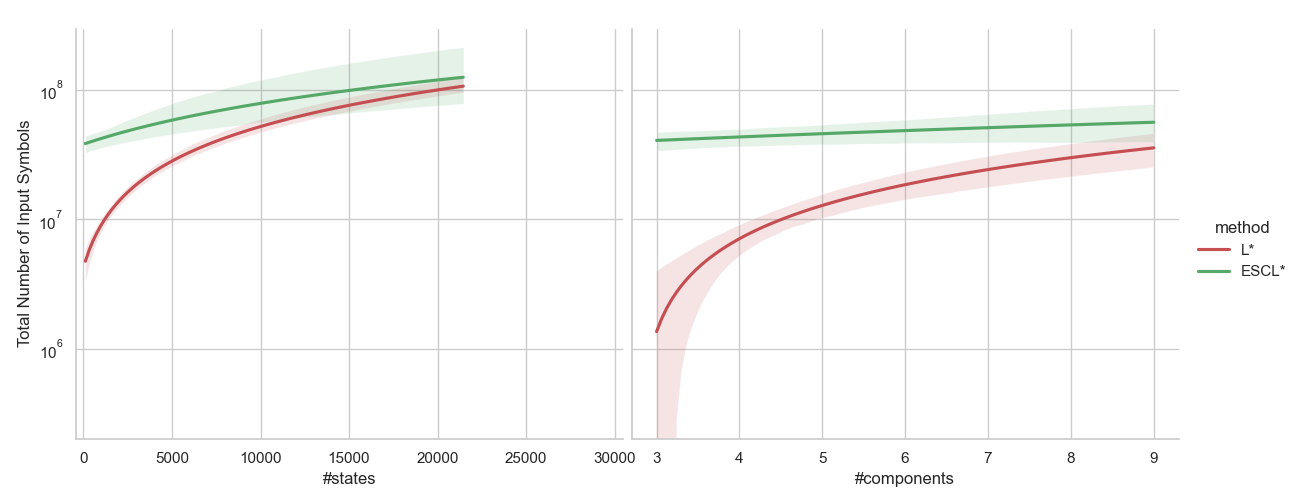
\includegraphics[width=0.48\textwidth]{Results/Plots/Symbols.png}\hfill
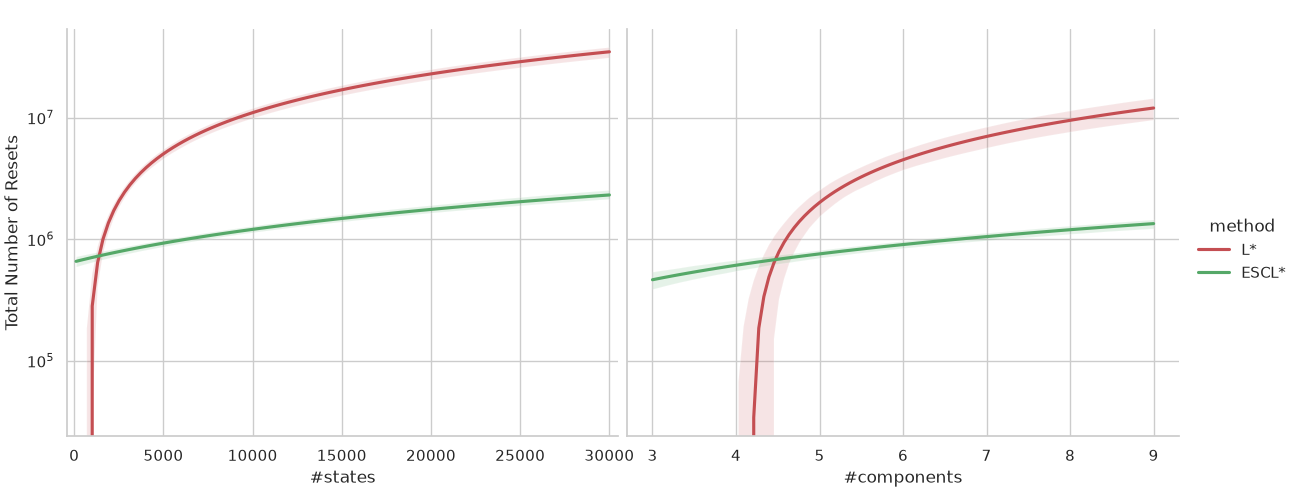
\includegraphics[width=0.48\textwidth]{Results/Plots/Resets.png}
\caption{مقایسه‌ی تعداد نمادهای پرسش عضویت (چپ) و تعداد بازنشانی‌ها (راست) برای \lr{LSTAR} در برابر \lr{ESCL-Star} روی مجموعه‌ی ادغام‌شده‌ی آزمون‌های تولیدشده.}
\label{fig:generated-plots}
\end{figure}

\section{بنچمارک واقعی: \lr{bankCard}}\label{sec:bankcard}
در گام پایانی، به‌جای تکیه‌ی صرف بر آزمون‌های تولیدشده، مجموعه‌ای از مدل‌های واقعیِ آموخته‌شده از پروتکل کارت‌های بانکی\LTRfootnote{bankCard} به‌عنوان بنچمارک جدید انتخاب شد. این مجموعه شامل ۱۱ مؤلفه است که هرکدام رفتارِ یک نوع کارت یا برنامه‌ی کاربردیِ بانکی (از جمله \lr{MasterCard}، \lr{MAESTRO}، \lr{PIN}، \lr{SecureCode}، و نمونه‌های \lr{ASN}، \lr{Rabo} و \lr{Volksbank}) را نمایش می‌دهند و جایگزینِ بنچمارک قبلی (مبتنی بر پروتکل \lr{BCS}) شدند. انتخاب \lr{bankCard} به این دلیل بود که کنش‌های اشتراکیِ چند مؤلفه در این پروتکل واقعی، نمونه‌ی طبیعی‌ای از کنش‌های هم‌گام‌ساز با خروجیِ وابسته به وضعیت هستند و بستری مناسب برای سنجشِ \lr{ESCL-Star} در شرایط واقعی فراهم می‌کنند.

علاوه بر این، برای افزایش جامعیتِ بنچمارک، به هر یک از مؤلفه‌های \lr{bankCard} یک کنش خصوصیِ (ناهم‌گام) اضافه شد تا هر مؤلفه، علاوه بر کنش‌های پروتکلیِ مشترک، حداقل یک رفتارِ محلی و غیرقابل‌مشاهده از بیرون نیز داشته باشد؛ این کار پوششِ بخشِ «خنثی‌سازی اثر کنش‌های خصوصی» (بخش \ref{sec:generator}) را در یک محیط واقعی نیز می‌آزماید. همچنین منطقِ انتخابِ زیرمجموعه‌ی مؤلفه‌ها برای هر آزمون (\lr{ChooseTests.py}) ساده‌سازی شد تا به‌جای گروه‌بندیِ از پیش تعیین‌شده‌ی مؤلفه‌های هم‌گام (که در بنچمارک \lr{BCS} استفاده می‌شد)، هر زیرمجموعه‌ای از مؤلفه‌های \lr{bankCard} بتواند در کنار هم آزموده شود.

جدول \ref{tab:bankcard-results} خلاصه‌ی نتایجِ اجرای \lr{ESCL-Star} روی این بنچمارک را در برابر بنچمارک واقعیِ پیشین نشان می‌دهد و شکل \ref{fig:bankcard-plots} نمودارهای مقایسه‌ای متناظر را نمایش می‌دهد.

\begin{table}[H]
\caption{میانگین معیارهای یادگیری روی بنچمارک واقعی: بنچمارک پیشین در برابر \lr{bankCard}}
\label{tab:bankcard-results}
\centering
\begin{tabularx}{\textwidth}{|X|r|r|r|r|}
\hline
\textbf{بنچمارک واقعی} & \textbf{\lr{LSTAR} (نماد)} & \textbf{\lr{CLSTAR} (نماد)} & \textbf{نسبتِ بهبود} & \textbf{تعداد آزمون} \\
\hline
بنچمارک پیشین (\lr{BCS}) & \lr{39{,}392{,}529} & \lr{20{,}321{,}058} & $\times 1.9$ & \lr{227} \\
\lr{bankCard} (تازه، با کنش خصوصیِ افزوده) & \lr{70{,}189{,}184} & \lr{28{,}054{,}821} & $\times 2.5$ & \lr{147} \\
\hline
\end{tabularx}
\end{table}

\begin{figure}[H]
\centering
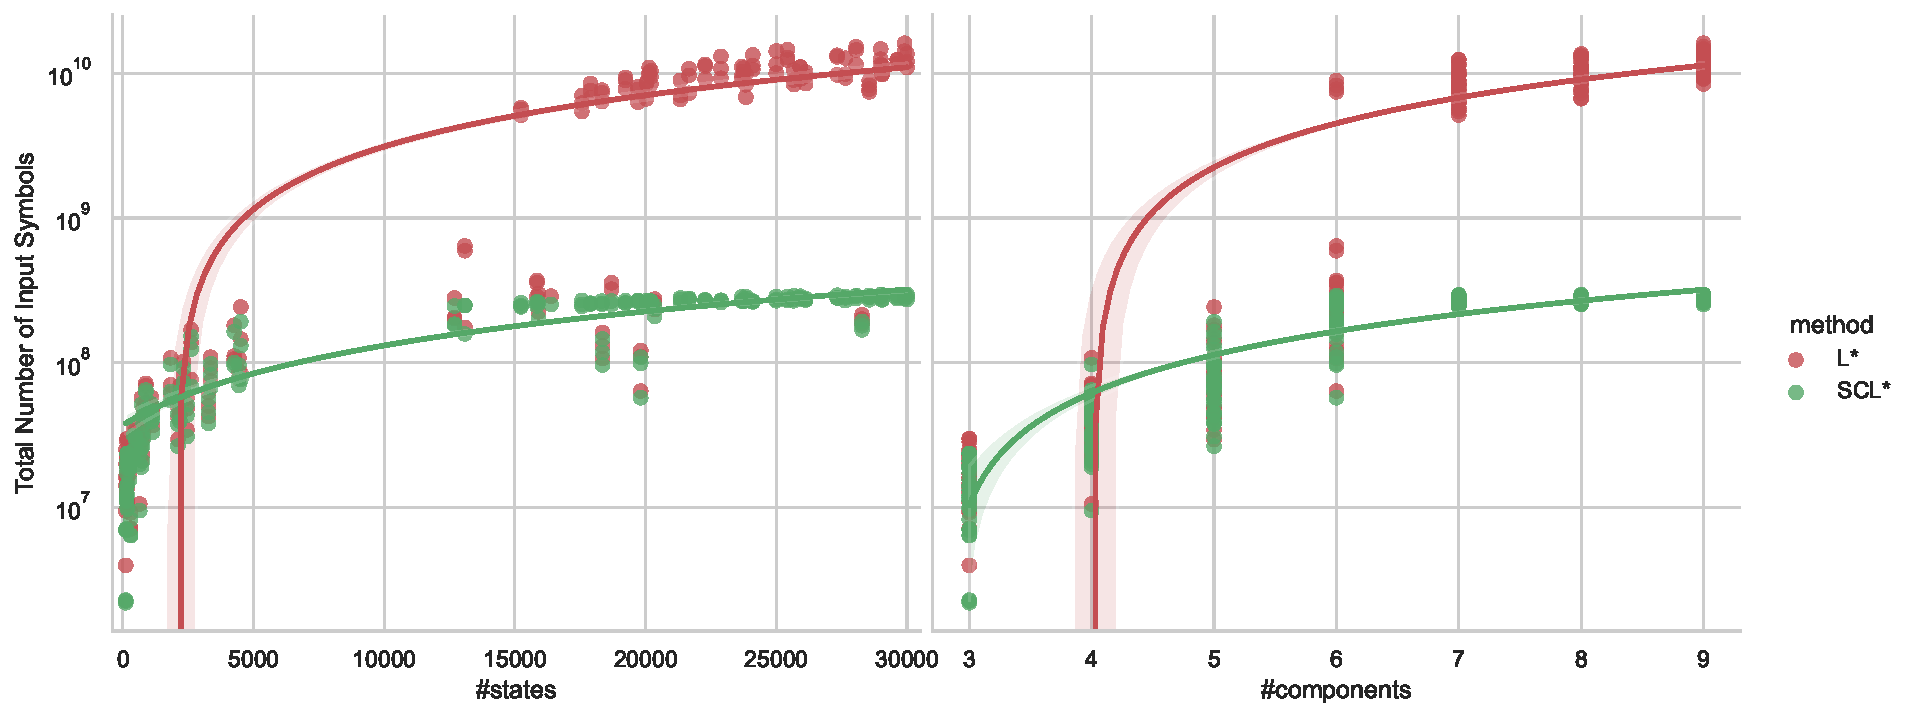
\includegraphics[width=0.32\textwidth]{Results/Plots/Real-Symbols.png}\hfill
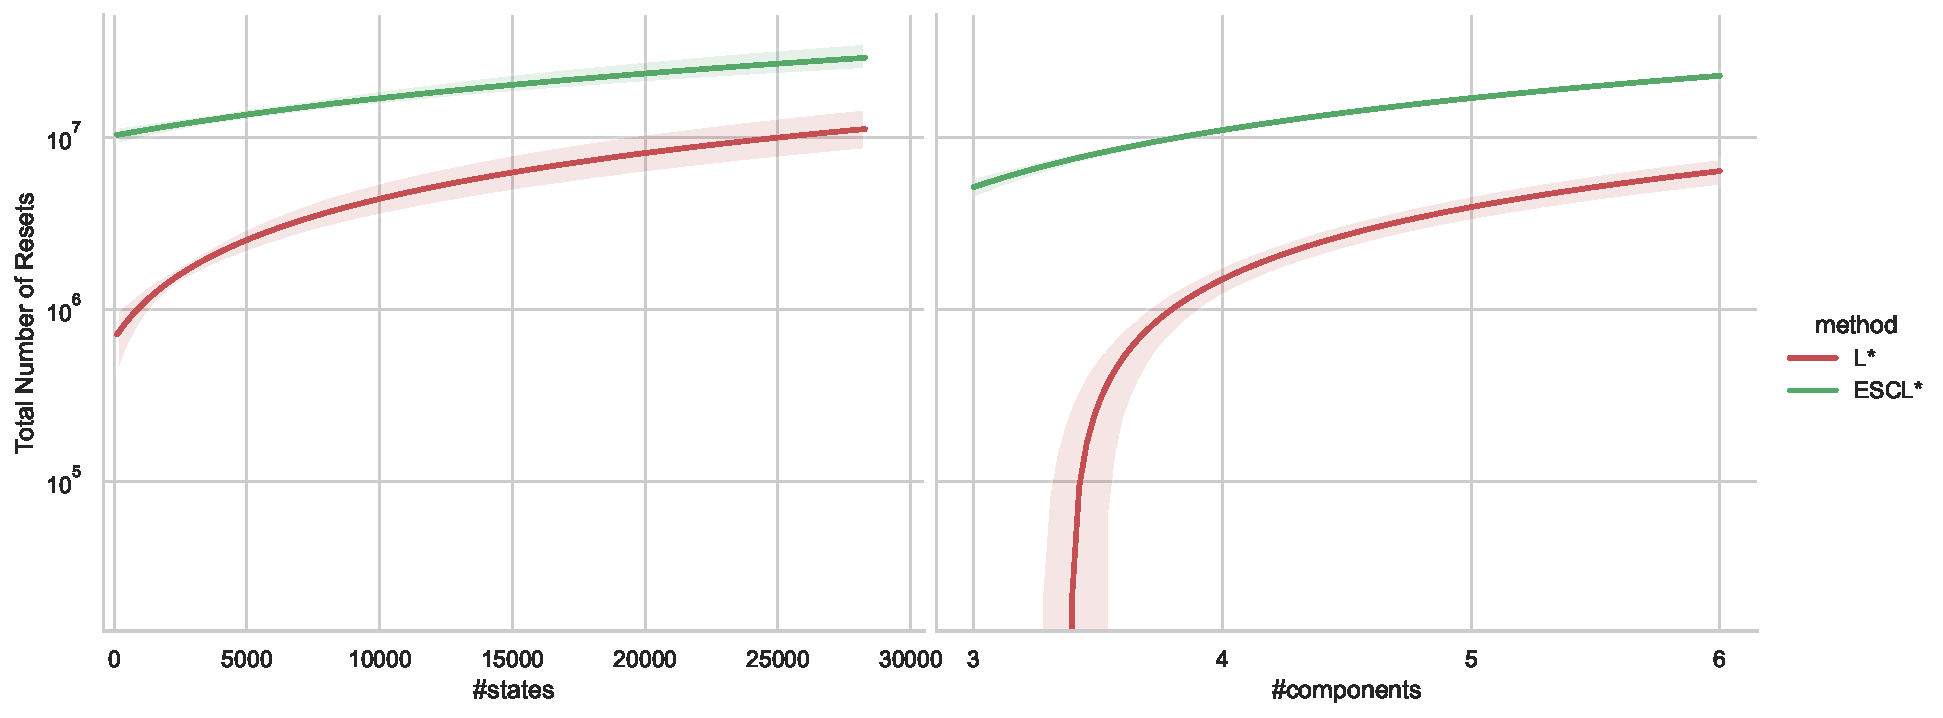
\includegraphics[width=0.32\textwidth]{Results/Plots/Real-Resets.png}\hfill
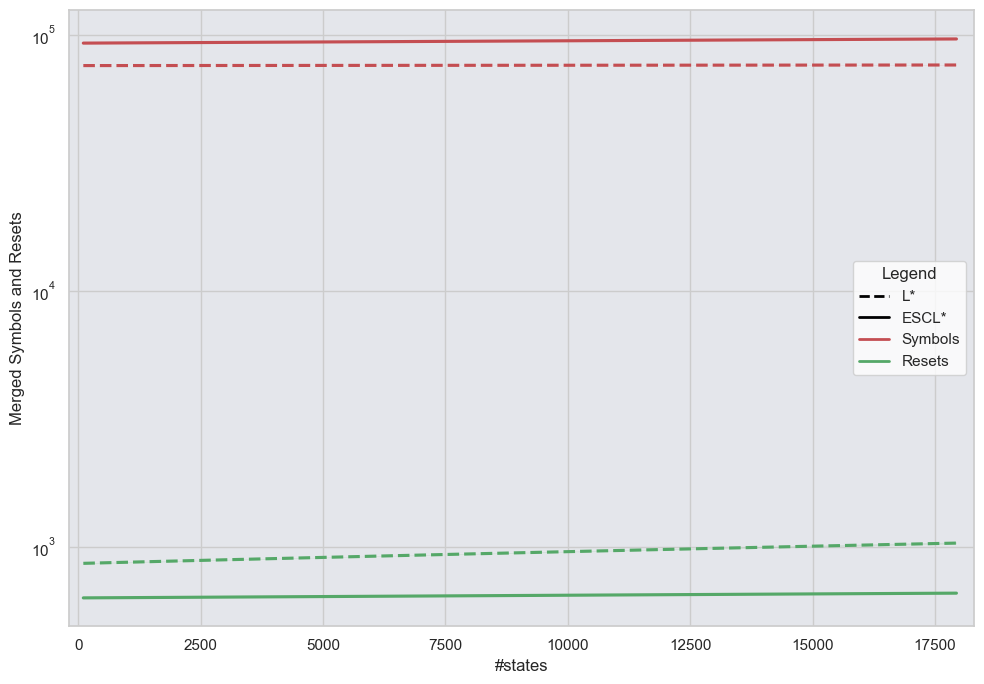
\includegraphics[width=0.32\textwidth]{Results/Plots/Real-Merged-Single-Plot.png}
\caption{نمودارهای مقایسه‌ی تعداد نمادها، تعداد بازنشانی‌ها، و نمای ادغام‌شده برای \lr{ESCL-Star} روی بنچمارک واقعیِ \lr{bankCard}.}
\label{fig:bankcard-plots}
\end{figure}

همان‌گونه که در جدول \ref{tab:bankcard-results} دیده می‌شود، بنچمارک \lr{bankCard} به‌دلیل بزرگ‌تر بودن مؤلفه‌ها (تعداد حالت‌ها معمولاً بین $140$ تا $224$) و افزودنِ کنش خصوصی به هر مؤلفه، هزینه‌ی مطلق یادگیری را نسبت به بنچمارک پیشین افزایش داده است؛ اما نسبتِ بهبودِ یادگیریِ ترکیبی نسبت به یادگیریِ یکپارچه ($\times 2.5$) نه‌تنها حفظ، بلکه نسبت به بنچمارک قبلی ($\times 1.9$) بهبود یافته است. این نتیجه نشان می‌دهد در سامانه‌های واقعیِ بزرگ‌تر و پیچیده‌تر، مزیتِ رویکرد ترکیبیِ \lr{ESCL-Star} پررنگ‌تر می‌شود.

\section{جمع‌بندی}
در این گزارش، توسعه‌ی الگوریتم \lr{SCL-Star} به \lr{ESCL-Star} برای پشتیبانی از کنش‌های هم‌گام‌سازِ با خروجیِ پویا (اما سازگار در نقاط هم‌گامی) شرح داده شد. تغییر اصلیِ سمتِ یادگیری، جایگزینیِ قاعده‌ی «حذفِ فوریِ کنش از \lr{sync} به‌محض مشاهده‌ی خروجیِ متفاوت» با رویه‌ای مبتنی بر یادگیریِ جزئی و بررسیِ صحتِ هم‌گامی در \lr{ProductMealy} بود. سمتِ دوم و دشوارترِ کار، تعمیمِ تولیدکننده‌ی آزمون‌های خودکار بود تا بتواند مؤلفه‌های تصادفیِ متنوعی تولید کند که رَدِ خروجیِ کنش هم‌گام‌سازشان، صرف‌نظر از تفاوتِ توپولوژی و اندازه، دقیقاً با یک الگوی مشترکِ (پیشوند $+$ دوره‌ی تناوب) منطبق بماند؛ حتی هنگام افزودنِ حالت‌ها و کنش‌های خصوصیِ اضافی. نتایج آزمایش‌ها، هم روی آزمون‌های تولیدشده و هم روی بنچمارک واقعیِ \lr{bankCard}، نشان داد که مزیتِ یادگیریِ ترکیبی نسبت به یادگیریِ یکپارچه، پس از این تعمیم همچنان حفظ می‌شود.

\end{document}
